\documentclass{article}
\usepackage{amsmath}
\usepackage{amsthm}
\usepackage{pgfplots}
\usepackage[margin=1in]{geometry}
\usepackage{listings}
\begin{document}
\begin{flushright}MAT 128A: Homework 2\\ Hangshi Jin\\ 913142686\\ Rohit Thomas
\end{flushright}
\begin{large}Section 3.2\end{large}
\\\\6.\[P_{1,2}=\frac{x-0.7}{0.4-0.7}\cdot2.8+\frac{x-0.4}{0.7-0.4}\cdot P_2=\frac{28}{15}+\frac{P_2}{3}\]
\[P_{0,1,2}=\frac{x-0.7}{0-0.7}\cdot3.5+\frac{x-0}{0.7-0}\cdot P_{1,2}=1+\frac{28}{21}+\frac{5P_2}{21}=\frac{27}{7}\]
\[\Rightarrow P_2=6.4\]
\begin{large}Section 3.3\end{large}
\\\noindent\rule{16cm}{0.4pt}\lstinputlisting[language=Matlab]{newton.m}\noindent\rule{16cm}{0.4pt}
\\8.
\\\\By using newton.m, we get
\\\\	a.
\[P_4(x)=1.0517*x + 0.5725*x*(x - 0.1) + 0.215*x*(x - 0.3)*(x - 0.1) + 0.06301587*x*(x - 0.3)*(x - 0.6)*(x - 0.1) - 6.0\]
b.
\[P_5(x)=1.0517*x + 0.5725*x*(x - 0.1) + 0.215*x*(x - 0.3)*(x - 0.1) + 0.06301587*x*(x - 0.3)*(x - 0.6)*(x - 0.1)\]\[ + 0.01415945*x*(x - 1.0)*(x - 0.3)*(x - 0.6)*(x - 0.1) - 6.0\]
10.
\\\\By using newton.m, we get
\[P(x)=3.0*x + (x + 1.0)*(2.0*x + 4.0) - 1.0*x*(x + 1.0)*(x + 2.0) + 7.0\]
\begin{flushright}which is of degree 3.\end{flushright}
11.
\\\\a.\\\\By using newton.m, we get
\[4.0*x - 1.0*(x + 1.0)*(3.0*x + 6.0) + x*(x + 1.0)*(x + 2.0) + 7.0=Q(x)\]
$\Rightarrow$ Q(x) interpolates the data.
\\\\Expand Q(x) and P(x), we get
\[P(x)=x^3 - 3.0*x + 1.0=Q(x)\]
$\Rightarrow$ P(x) also interpolates the data.
\\\\We can also plug in x into both P(x) and Q(x) to see if they equal to y, which also tells they interpolate the data.
\\\\b.
\\\\Because P(x) and Q(x) are resulted from two different methods with different formats, where P(x) has a catastrophic cancellation for degree 2 term.
\\\\\begin{large}Section 3.4\end{large}
\\\noindent\rule{16cm}{0.4pt}\lstinputlisting[language=Matlab]{Hermite.m}\noindent\rule{16cm}{0.4pt}
\\\\2.c.
\\\\By using Hermite.m, we get
\[H_5(x)=(0.945237*x - 0.0945237)*(x - 0.1) - 2.801997*x - 1.0*(0.47935*x - 0.047935)*(x - 0.1)*(x - 0.2)^2 \]\[- 1.0*(x - 0.1)*(x - 0.2)*(0.297*x - 0.0297) - 1.0*(x - 0.3)*(x - 0.1)*(x - 0.2)^2*(1299.972*x - 129.9972) - 0.00985021
\]
6.\[f'(x)=-2e^{2x}+3xe^x+3e^x,f(x_0)=3e^1 - e^2,f(x_1)=3.15e^{1.05} - e^{2.1}\]
a.\\\\By using Hermite.m, we get
\[H_3(x)=1.531579*x - 1.0*(x - 1.0)*(174.234*x - 174.234) + (6853.612*x - 6853.612)*(x - 1.0)*(x - 1.05) - 0.7657894\]
\[H_3(1.03)=0.8093248562,R_3(x)=\frac{-e^x\cdot(16e^x-3x-12)}{4\cdot3\cdot2}\left(x-1\right)^2\left(x-1.05\right)^2\]
\[\text{Error bound}\leq\left|\frac{-e^{1.025}\cdot(16e^{1.025}-3\cdot1.025-12)}{4\cdot3\cdot2}\left(1.025-1\right)^2\left(1.025-1.05\right)^2\right|=0.00000133904546929\]
\[\text{actual error}=|f(1.03)-H_3(1.03)|=0.00000123731717216<0.00000133904546929\]
10.a.\\\\By using Hermite.m, we get
\[H_9(x)=75.0*x + 0.2222222*x^2*(x - 3.0) - 0.03111111*x^2*(x - 3.0)^2 + 0.002263889*x^2*(x - 5.0)^2*(x - 3.0)^2 \]\[- 0.006444444*x^2*(x - 5.0)*(x - 3.0)^2 - 0.0009131944*x^2*(x - 8.0)*(x - 5.0)^2*(x - 3.0)^2\]\[ + 0.0001305268*x^2*(x - 8.0)^2*(x - 5.0)^2*(x - 3.0)^2 - 0.00002022363*x^2*(x - 8.0)^2*(x - 5.0)^2*(x - 3.0)^2*(x - 13.0)
\]
\[H_9(10)=742.50283909877\]
\begin{center}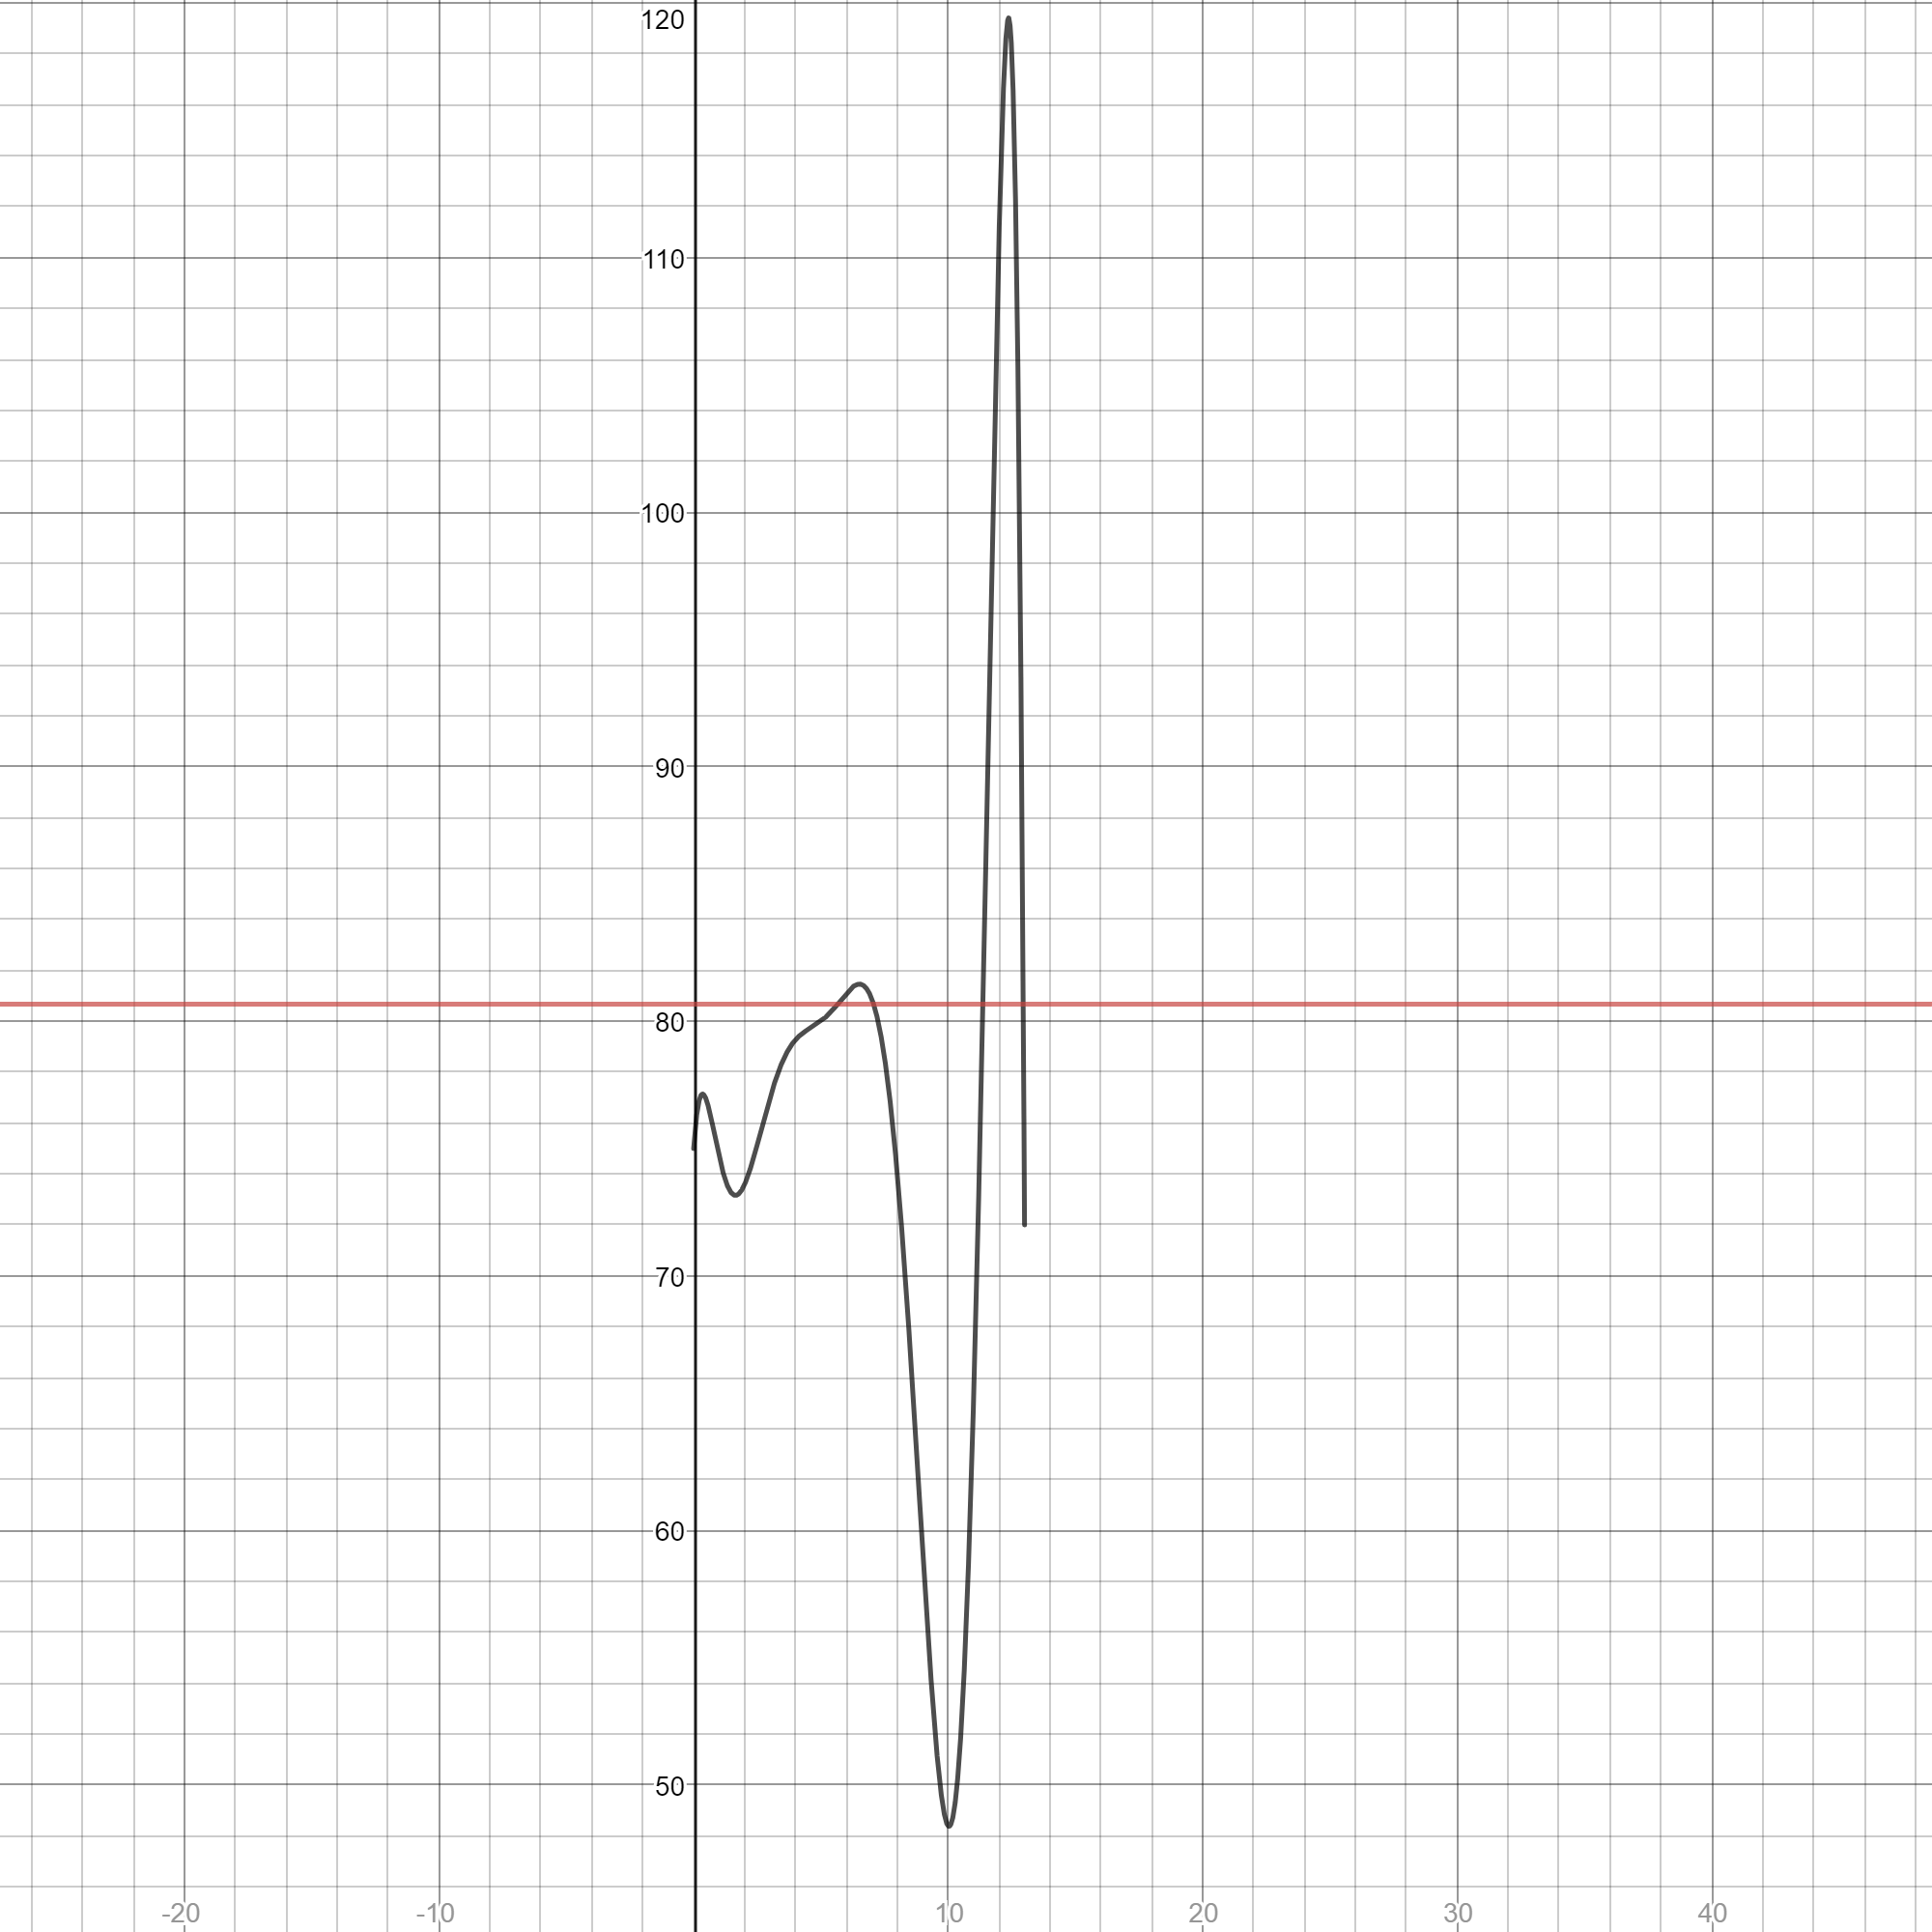
\includegraphics[width=0.5\textwidth]{10}\end{center}
b.\[55mi/hr=80.67ft/sec\]
Through the graph, we see the car exceeds 55mi/hr first at x=5.651sec.\\\\
c.\\\\Through the graph, we see the approximate maximum speed for the car is 119.417ft/sec=81.421mi/hr at t=12.372s.
\\\\\begin{large}Section 3.5\end{large}
\\\noindent\rule{16cm}{0.4pt}\lstinputlisting[language=Matlab]{cpsplinecalc.m}\noindent\rule{16cm}{0.4pt}
\\\\2.
\\\\By using cpsplinecalc.m, we get\[s_0(x)=s_1(x)=x\]
\\\noindent\rule{16cm}{0.4pt}\lstinputlisting[language=Matlab]{psplinecalc.m}\noindent\rule{16cm}{0.4pt}
\\\\4.c.\\\\By using psplinecalc.m, we get
\[s_0(x) =4.38125*(x - 0.1)^3 - 2.751286*x - 0.01492133\]\[
s_1(x) =1.314375*(x - 0.2)^2 - 2.619849*x - 4.38125*(x - 0.2)^3 - 0.03682758\]
8.c.
\\\\By using cpsplinecalc.m, we get
\[s_0(x) =12.81506*(x - 0.1)^3 - 0.3512485*(x - 0.1)^2 - 2.8005*x - 0.01\]
\[s_1(x) =3.493271*(x - 0.2)^2 - 2.486297*x - 39.52535*(x - 0.2)^3 - 0.06353787\]
14.\[s_0(1)=1+B=1=s_1(1),\Rightarrow B=0, s'_0(1)=B-2=b=s_1'(1),\Rightarrow b=-2\]
\[\Rightarrow f'(0)=s'_0(0)=B=0,f'(2)=s'_1(2)=b+13=11\]
16.
\[y=[1 e^{-0.25} e^{-0.75} e^{-1}]\]
By using psplinecalc.m, we get
\[s_0(x) =0.6208652*x^3 - 0.9236009*x + 1.0\]
\[s_1(x)=0.4656489*(x - 0.25)^2 - 0.8071887*x - 0.1540168*(x - 0.25)^3 + 0.980598\]
\[s_2(x)=0.2346237*(x - 0.75)^2 - 0.4570524*x - 0.3128316*(x - 0.75)^3 + 0.8151559\]
\[\text{approx}=\int_0^{0.25}s_0(x)dx+\int_{0.25}^{0.75}s_1(x)dx+\int_{0.75}^1s_2(x)dx=0.631966361168031\]
\[s'(0.5)=s'_1(0.5)=-0.6032424115,s''(0.5)= s''_1(0.5)=0.7002726321541\]
\[\text{actual}=\int_0^1e^{-x}dx=0.63212055882,f'(0.5)=-e^{-0.5}=-0.60653065971263<s'(0.5),f''(0.5)=e^{-0.5}=0.60653065971263<s''(0.5)\]
18.
\\\\Use cpsplinecalc.m, we get
\[s_0(x) =- 0.154515*x^3 + 0.4994413*x^2 - 1.0*x + 1.0\]
\[s_1(x) =0.383555*(x - 0.25)^2 - 0.7792509*x - 0.1015802*(x - 0.25)^3 + 0.9736135\]
\[s_2(x) =0.2311847*(x - 0.75)^2 - 0.471881*x - 0.06181745*(x - 0.75)^3 + 0.8262773\]
\[\text{approx}=\int_0^{0.25}s_0(x)dx+\int_{0.25}^{0.75}s_1(x)dx+\int_{0.75}^1s_2(x)dx=0.63207773208960\]
\[s'(0.5)=s'_1(0.5)=-0.60651969936339,s''(0.5)= s''_1(0.5)=0.61473976438377\]
\[\text{actual}=\int_0^1e^{-x}dx=0.63212055882,f'(0.5)=-e^{-0.5}=-0.60653065971263<s'(0.5),f''(0.5)=e^{-0.5}=0.60653065971263<s''(0.5)\]
19.Let\[f(x)=a+bx+cx^2+dx^3,\]
by the definition of a cubic spline interpolant S, f interpolates itself for $x_0...x_n$.
\\\\Since the property of clamped spline holds, f is its own clamped cubic spline.
\\\\$f''(x)=2c+6dx\Rightarrow f''(x)=0$ only at $x=\frac{-c}{3d}\neq x_0\neq x_n$. 
\\\\$\Rightarrow$ f cannot be a natural cubic spline.
\\\\29.a.
\\\\Use cpsplinecalc.m, we get
\[s_0(x)=0.219764*x^3 - 0.659292*x^2 + 75.0*x\]
\[s_1(x) =76.97788*x + 1.318584*(x - 3.0)^2 - 0.1537611*(x - 3.0)^3 - 5.933628\]
\[s_2(x) =80.40708*x + 0.3960177*(x - 5.0)^2 - 0.177237*(x - 5.0)^3 - 19.0354\]
\[s_3(x) =77.99779*x - 1.199115*(x - 8.0)^2 + 0.0799115*(x - 8.0)^3 - 0.9823009\]
\[S(10)=s_3(10)=774.838407079646\]
\begin{center}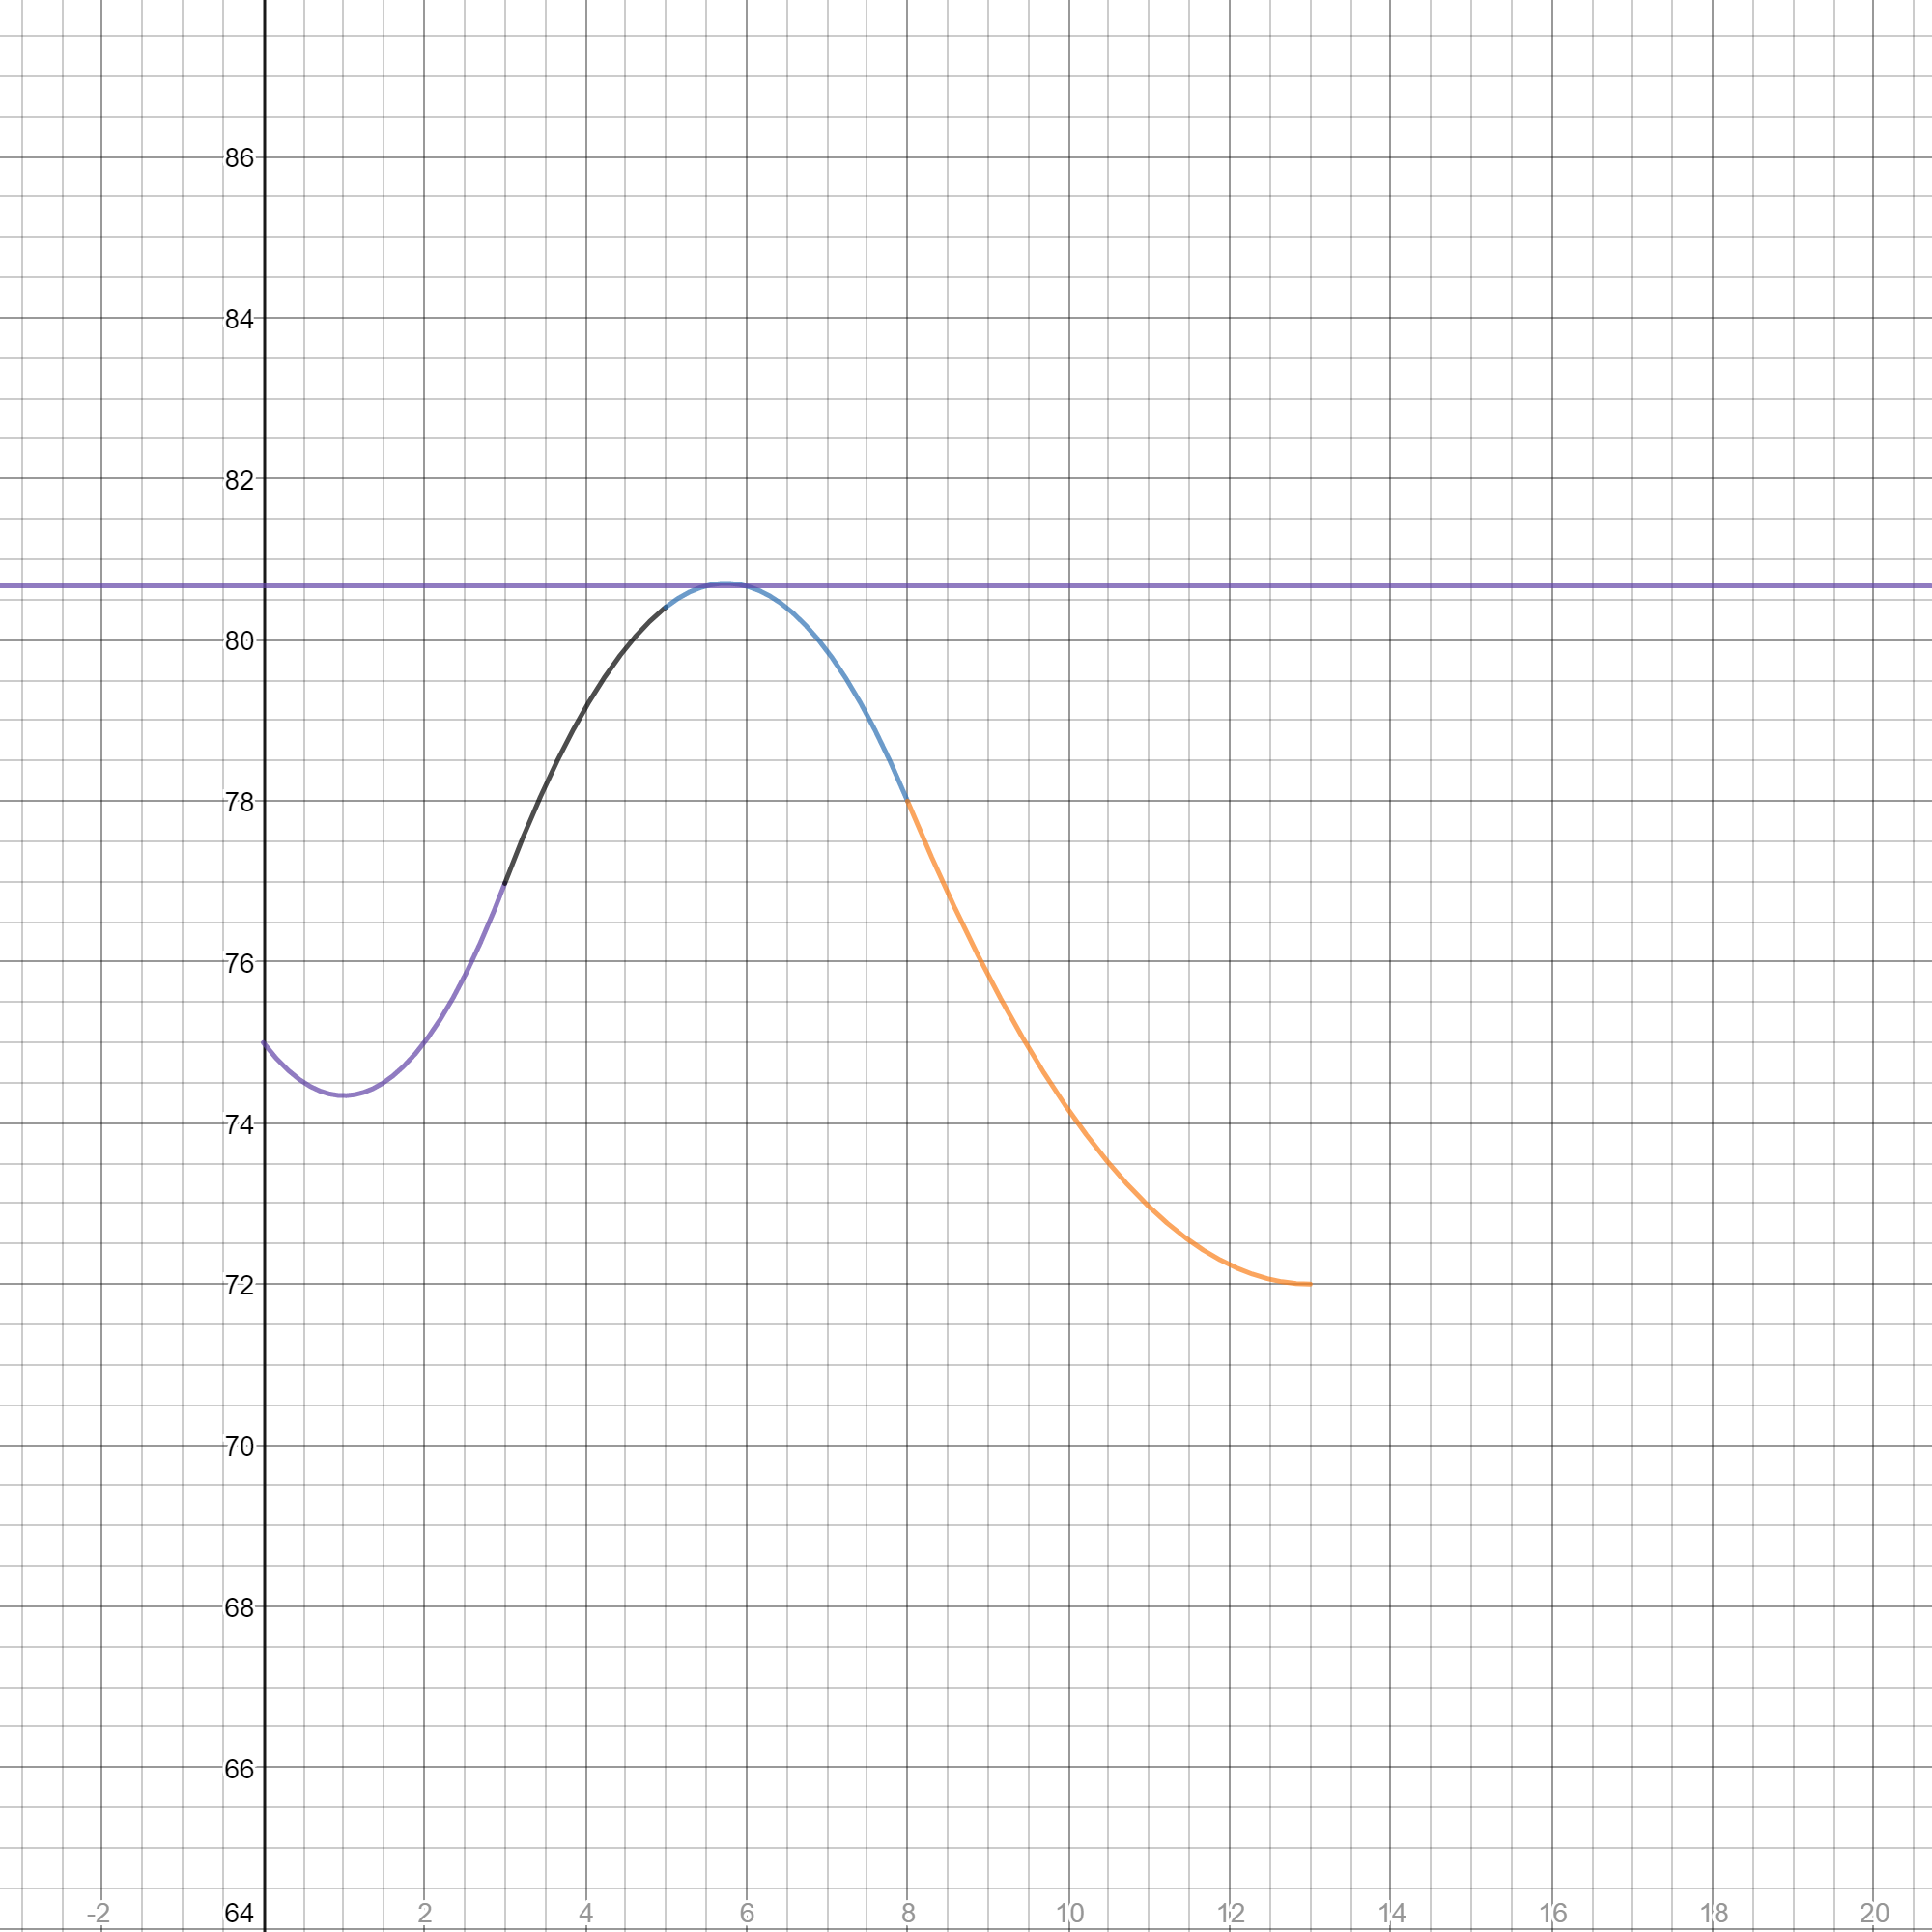
\includegraphics[width=0.5\textwidth]{29}\end{center}
b.\[55mi/hr=80.67ft/sec\]
Through the graph, we see the car exceeds 55mi/hr first at x=5.499sec.\\\\
c.\\\\Through the graph, we see the approximate maximum speed for the car is 80.702ft/sec=55.024mi/hr at t=5.745s.
\\\\\begin{large}Section 3.5\end{large}
\\\noindent\rule{16cm}{0.4pt}\lstinputlisting[language=Matlab]{parahermite.m}\noindent\rule{16cm}{0.4pt}
\\\\1.c.
\\\\By using parahermite.m, we get
\[x(t) =- 10*t^3 + 14*t^2 + t,y(t) =- 4*t^3 + 5*t^2 + t, \text{and clearly } 0\leq t\leq1\]
\begin{center}
   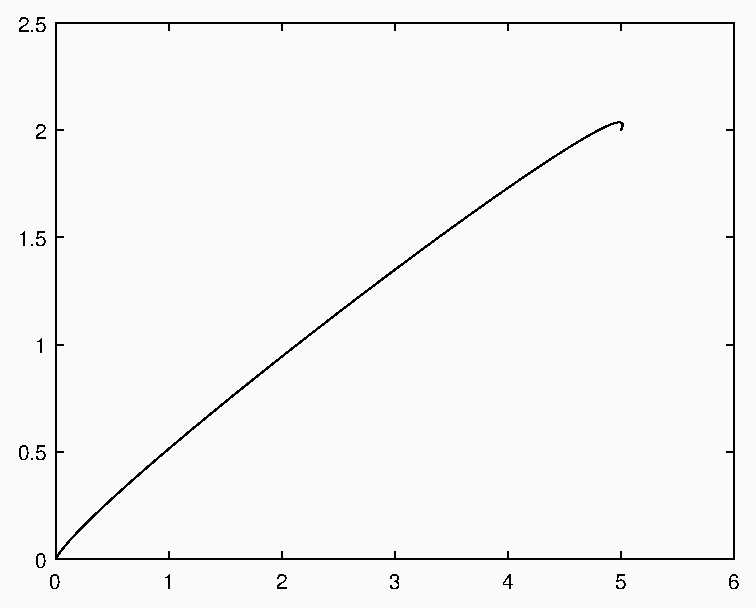
\includegraphics[scale=1]{2.eps}
\end{center}
\end{document}